\documentclass{article}
\usepackage[utf8]{inputenc}
\usepackage{graphicx}
\usepackage{caption}
\graphicspath{{q1_figs/}{q2a_figs/}{q2b_{figs}}}
\title{CS6910 Assignment 1}
\author{Lakshya J(EE19B035), Neham Jain(EE19B084), Nisharg Manvar(EE19B094)}
\date{March 2022}

\begin{document}

\maketitle

\section{Function Approximation Task}
In this task, we are asked to create a Multi Layer Feed Forward Neural Network of two layers where the Learning Rate and the number of neurons in each layer are hyper-parameters.\\
\\
We are supposed to use Stochastic Gradient Descent as the optimizer and Mean Squared Error Loss for the loss function.\\
$tanh$ was used as the activation function after every layer except for the last output layer.\\
\\
I ran the model for 2000 epochs on  batch sizes of 16, 32, 64, 128 for varying learning rates and number of neurons.\\
\\
Learning rates used: [1e-6, 1e-5, 1e-4, 1e-3, 1e-2]\\
Number of neurons: [50, 100, 256, 512, 784, 1024, 2048]\\
\\
Out of all these cases, I observed the least loss for the validation set in the case of batch size of 16, learning rate = 0.01 and number of neurons = 512.\\
\\
Here is the result obtained:\\
$Learning\ Rate:\ 0.01\\
No.\ of\ Neurons:\ 50\\
Validation\ loss:\ 0.0003136$\\
\\
I tested this model on the test set to obtain final results.
\\
\newpage
\subsection{Plots Obtained}
First, I plot the 3D plot of the actual function.
\begin{figure}[htbp]
    \centering
    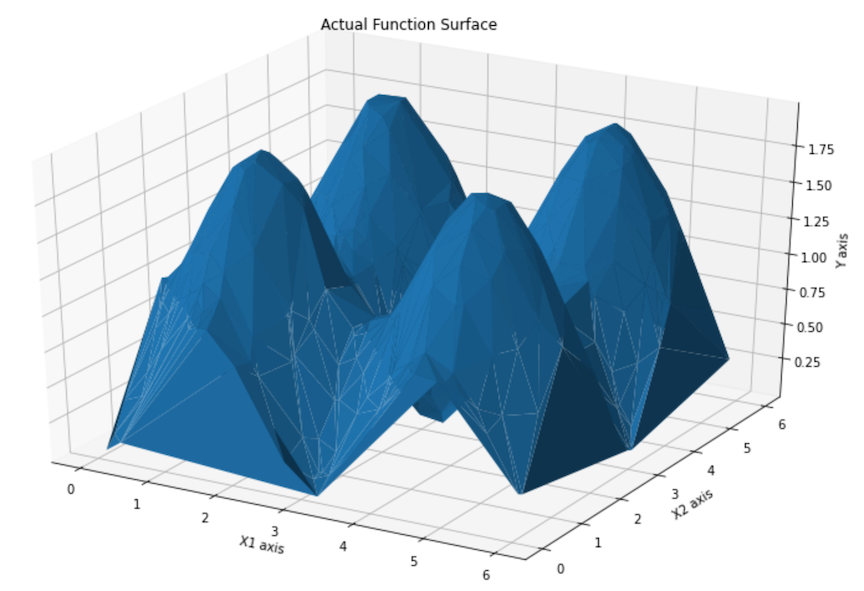
\includegraphics[width=0.8\linewidth]{ActualFunc.png}
    \captionsetup{justification=centering}
    \caption{Actual Plot}
\end{figure}
\\Next I plot the output obtained after training the model for various epochs. I plot the output of the model for epochs 1, 2, 10, 50, 500, 1000, 1500 and 2000(when the training is stopped).\\
It is observed that as the model moves through epochs, it is able to approximate the output better and give a smoother 3D output.
\begin{figure}[htbp]
    \centering
    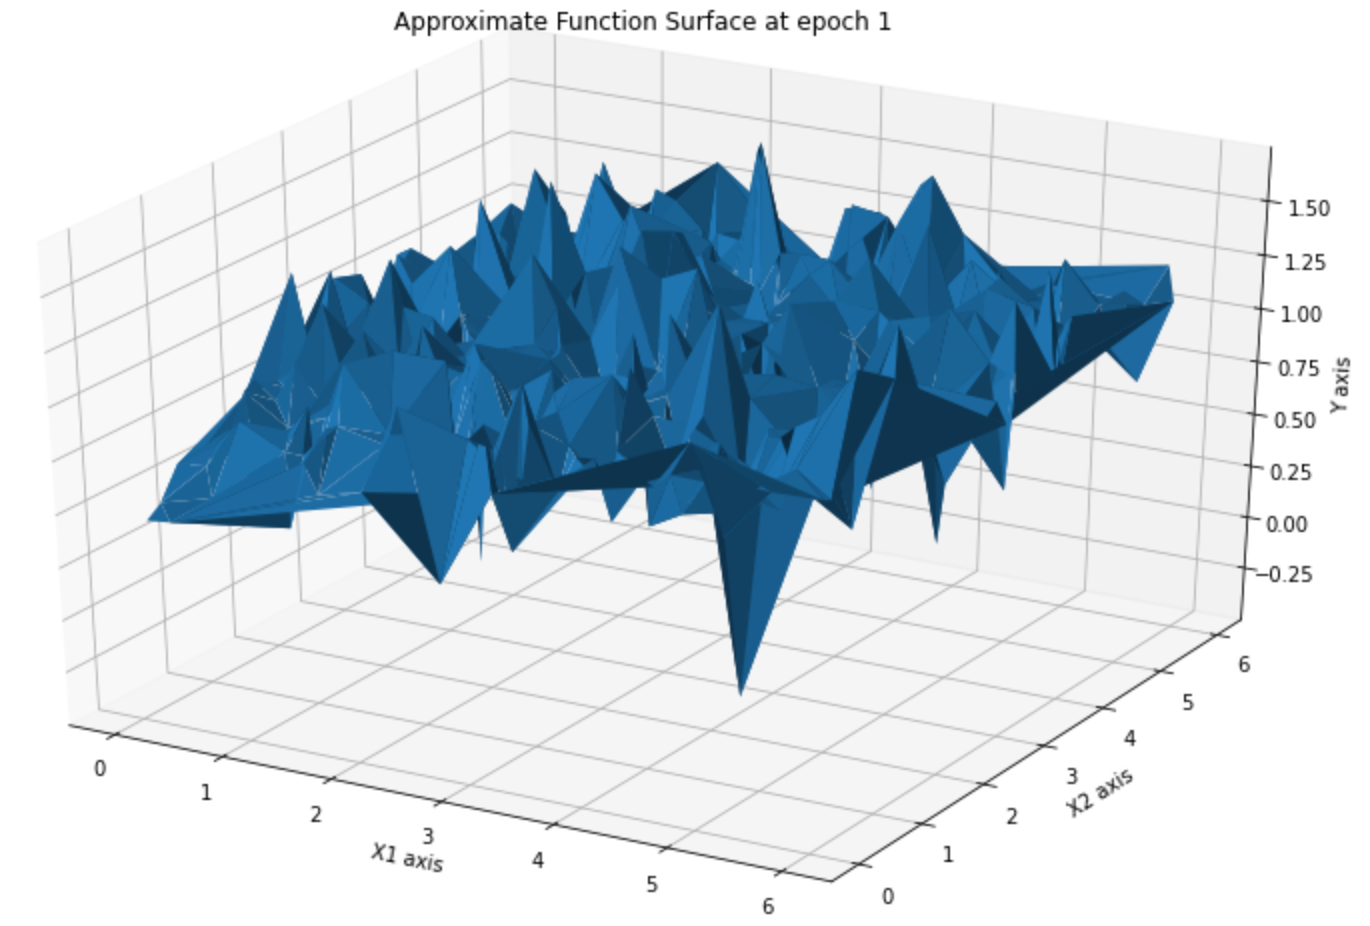
\includegraphics[width=0.8\linewidth]{Ep1.png}
    \captionsetup{justification=centering}
    \caption{Plot of all data applied on the model after 1 epoch}
\end{figure}
\begin{figure}[htbp]
    \centering
    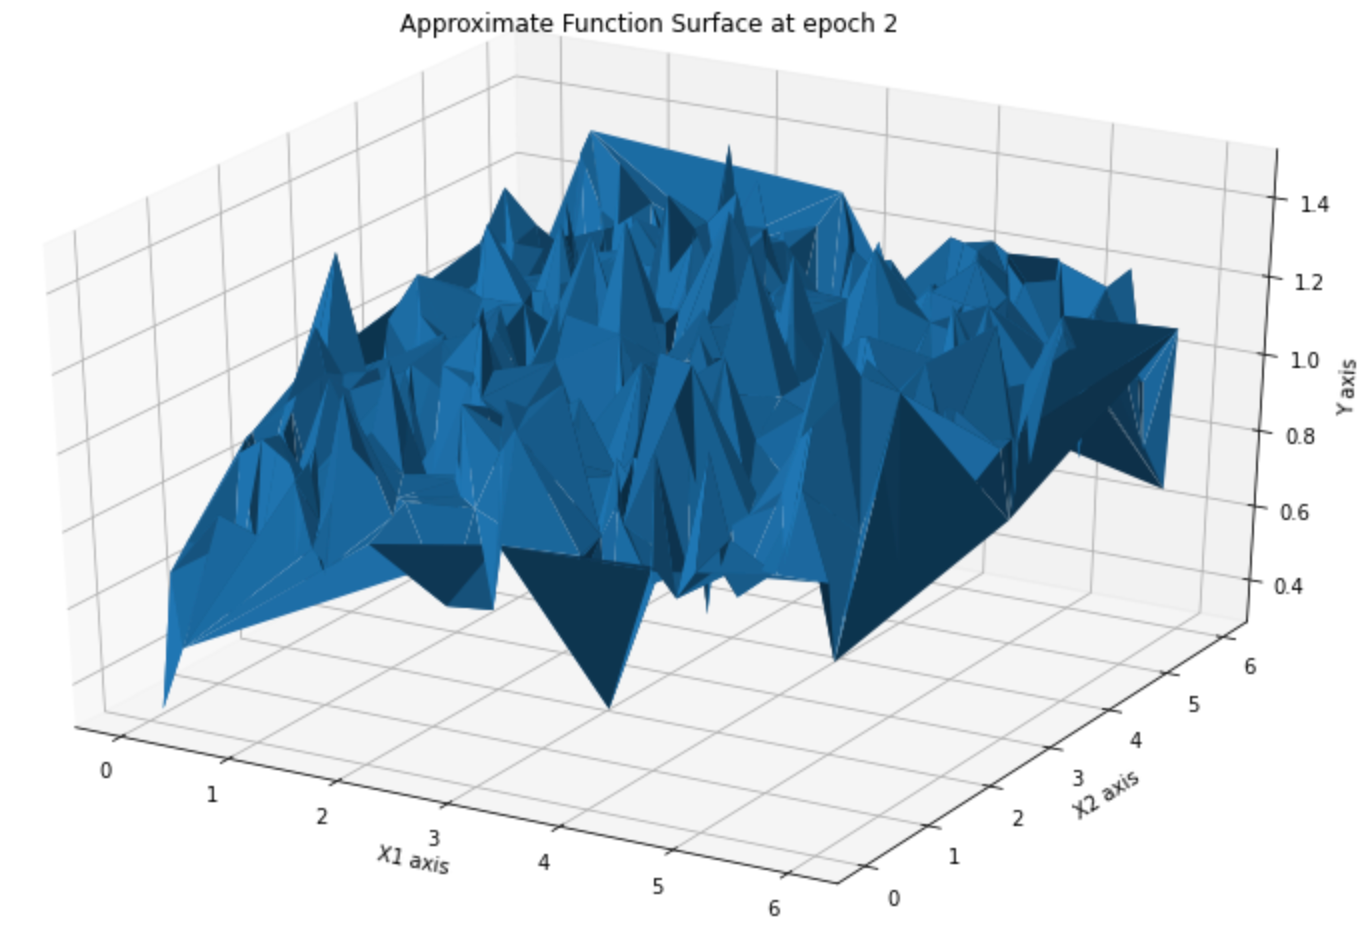
\includegraphics[width=0.8\linewidth]{Ep2.png}
    \captionsetup{justification=centering}
    \caption{Plot of all data applied on the model after 2 epoch}
\end{figure}
\begin{figure}[htbp]
    \centering
    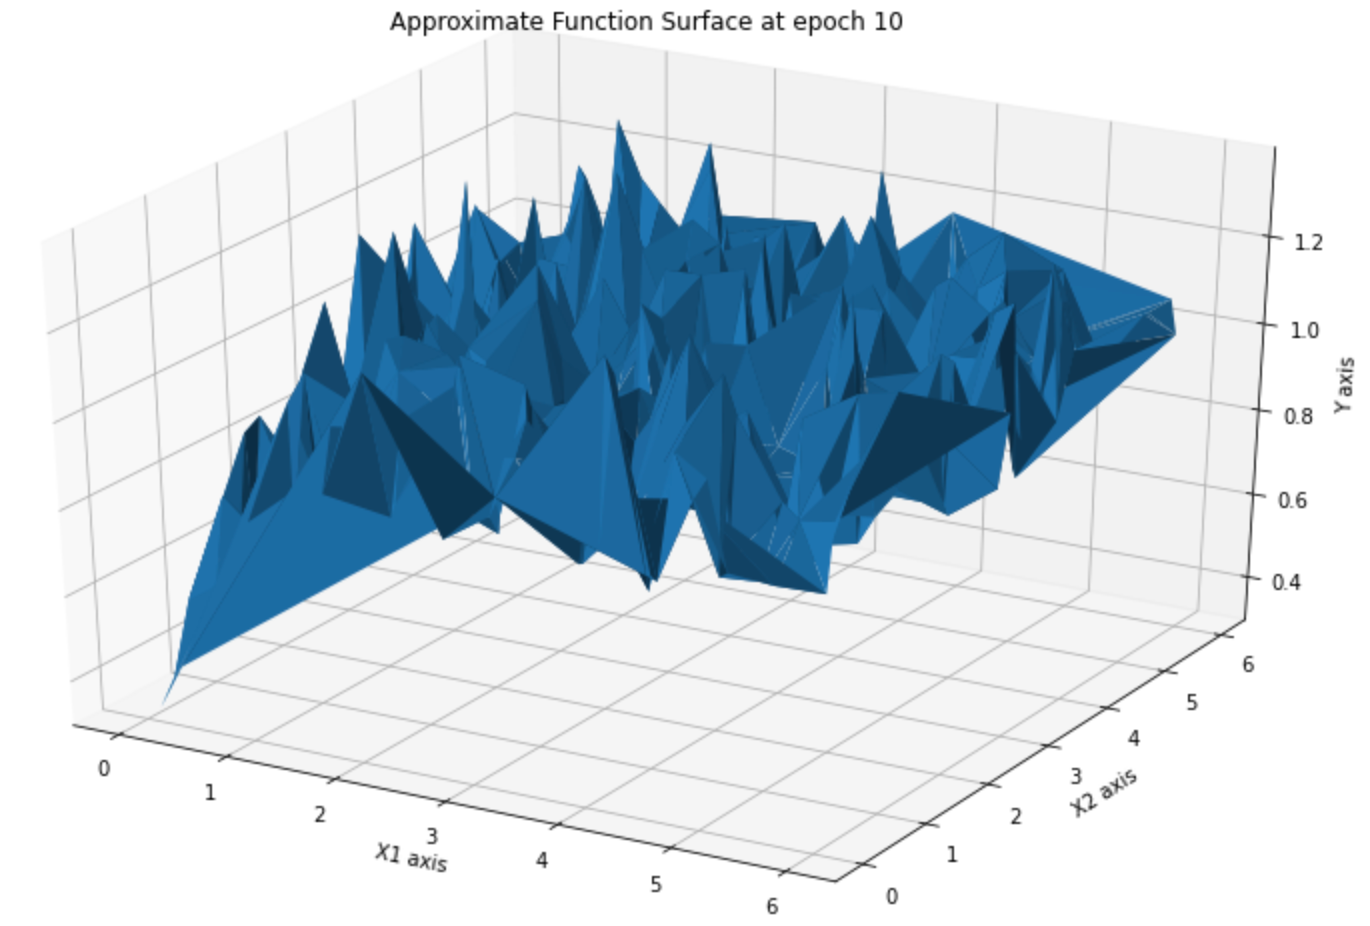
\includegraphics[width=0.8\linewidth]{Ep10.png}
    \captionsetup{justification=centering}
    \caption{Plot of all data applied on the model after 10 epoch}
\end{figure}
\begin{figure}[htbp]
    \centering
    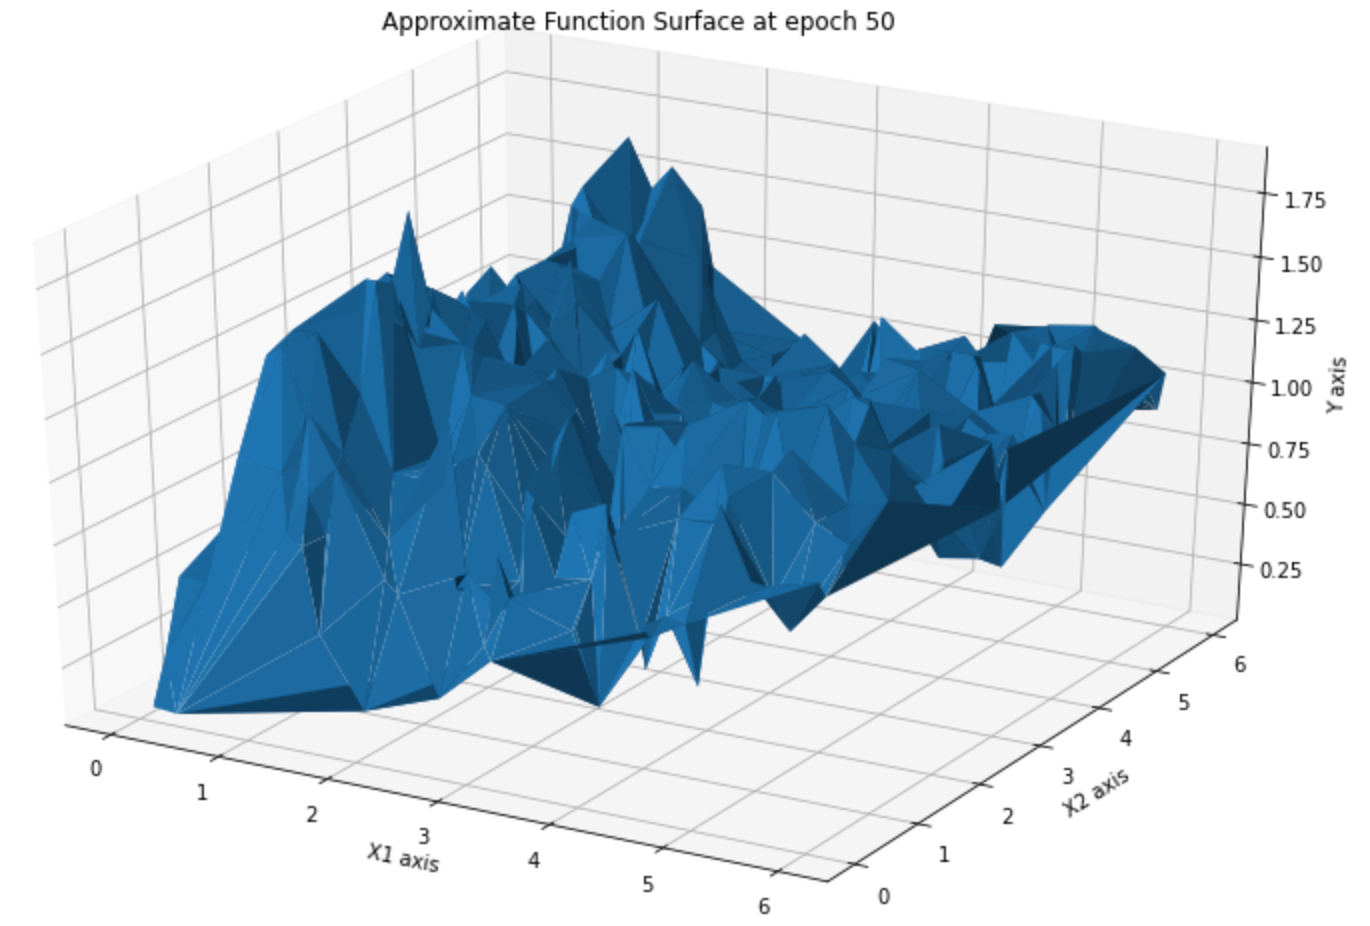
\includegraphics[width=0.8\linewidth]{Ep50.png}
    \captionsetup{justification=centering}
    \caption{Plot of all data applied on the model after 50 epoch}
\end{figure}
\begin{figure}[htbp]
    \centering
    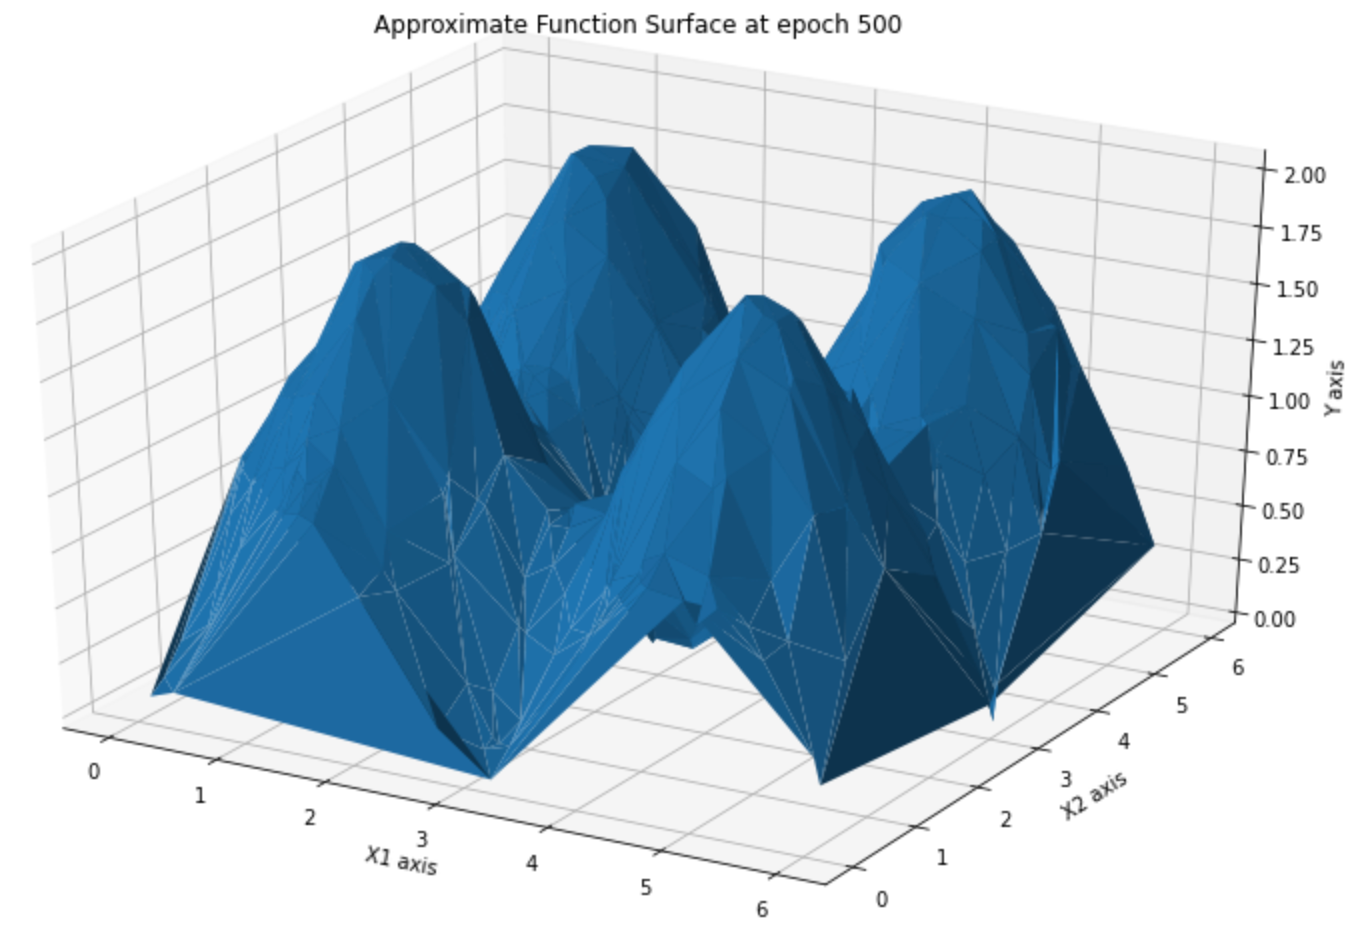
\includegraphics[width=0.8\linewidth]{Ep500.png}
    \captionsetup{justification=centering}
    \caption{Plot of all data applied on the model after 500 epoch}
\end{figure}
\begin{figure}[htbp]
    \centering
    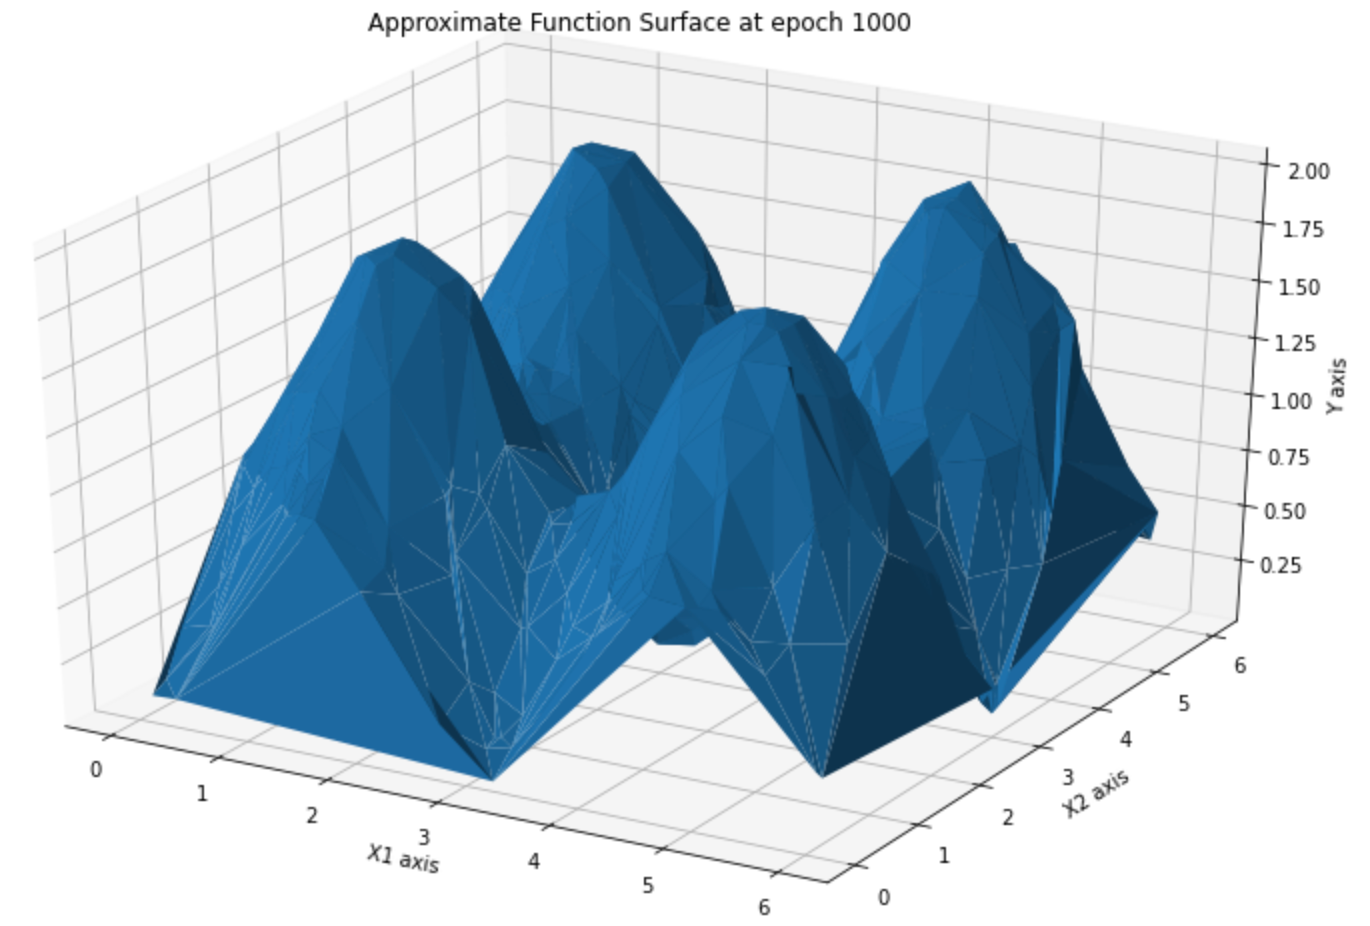
\includegraphics[width=0.8\linewidth]{Ep1000.png}
    \captionsetup{justification=centering}
    \caption{Plot of all data applied on the model after 1000 epoch}
\end{figure}
\begin{figure}[htbp]
    \centering
    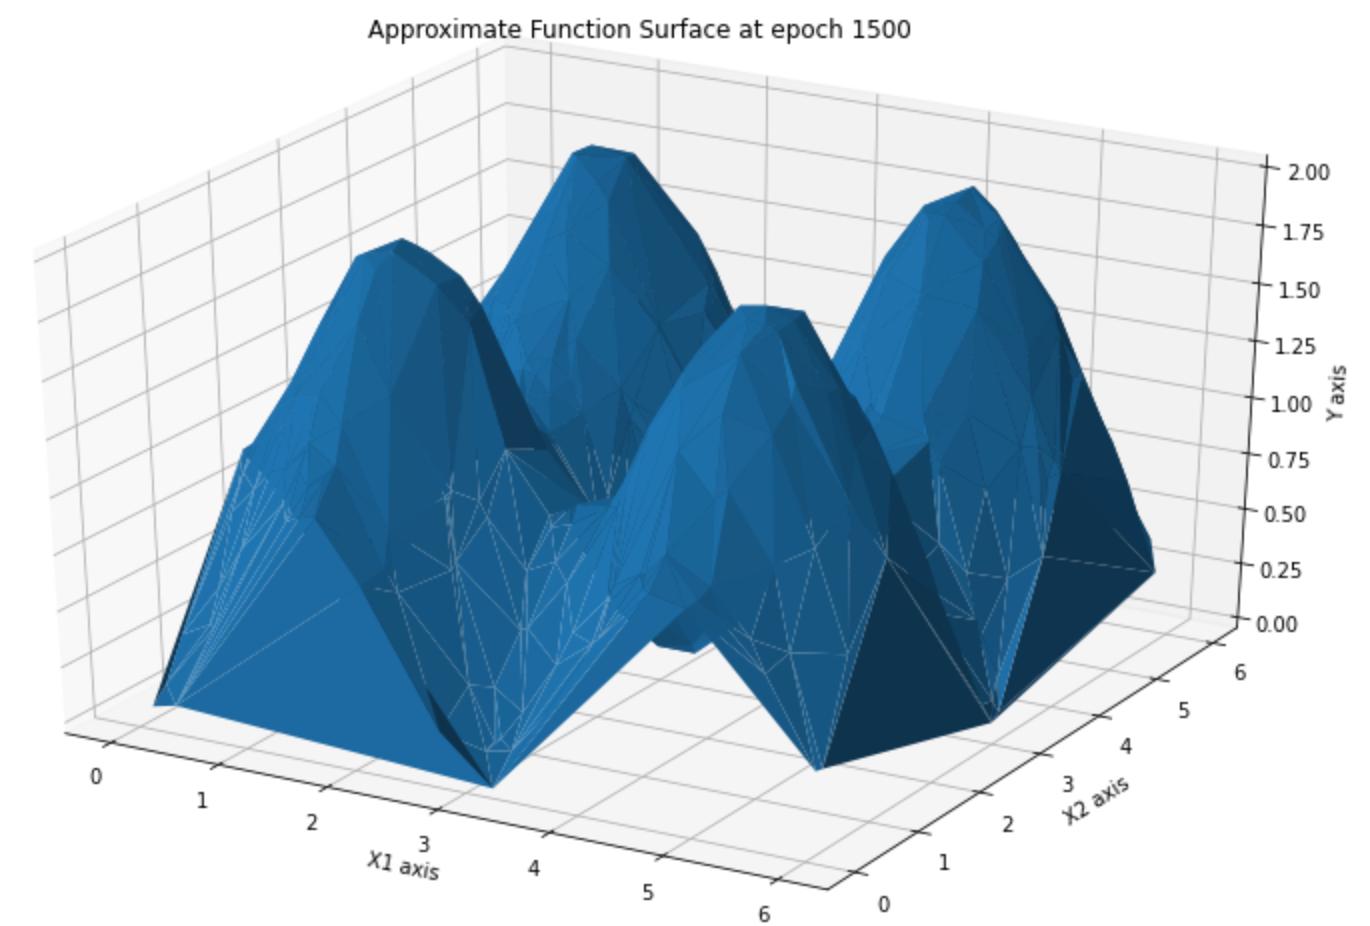
\includegraphics[width=0.8\linewidth]{Ep1500.png}
    \captionsetup{justification=centering}
    \caption{Plot of all data applied on the model after 1500 epoch}
\end{figure}
\begin{figure}[htbp]
    \centering
    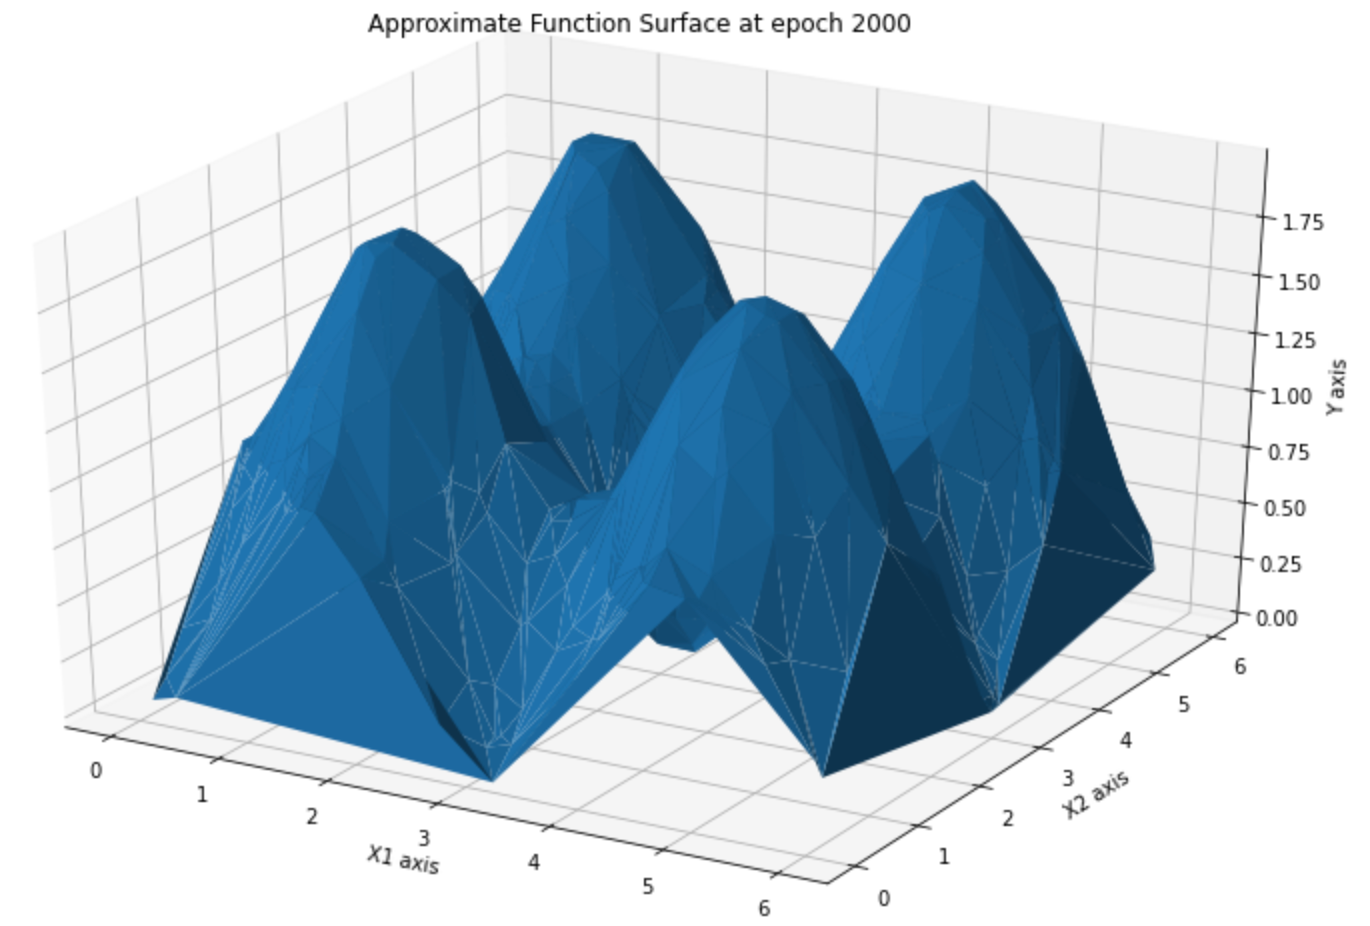
\includegraphics[width=0.8\linewidth]{Ep2000.png}
    \captionsetup{justification=centering}
    \caption{Plot of all data applied on the model after 2000 epoch}
\end{figure}
\newpage
Next I plot the error plot for the t

\subsection{Implementation Details:}

To prevent the model from overfitting (blah blah blah)


raining data, to see how well the training data learns with multiple epochs. We observe that the loss steeply drops within the first few epochs and them asymptotically reaches to a value after which it is not able to learn much, and oscillates around the found local optimum.
\begin{figure}[htbp]
    \centering
    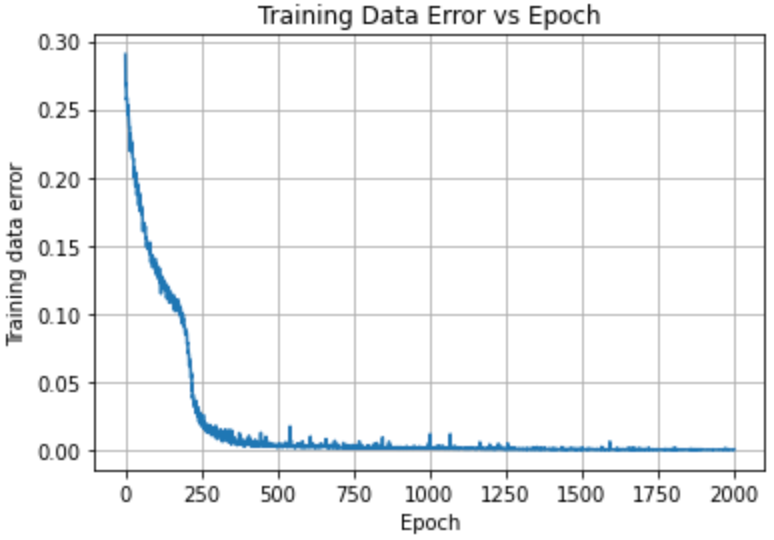
\includegraphics[width=0.8\linewidth]{errvsep.png}
    \captionsetup{justification=centering}
    \caption{Training data error vs Number of epochs}
\end{figure}
\\
The scatter plot after after training the model for 1500 epochs with the above parameters is as follows.\\
\\

\begin{figure}[htbp]
    \centering
    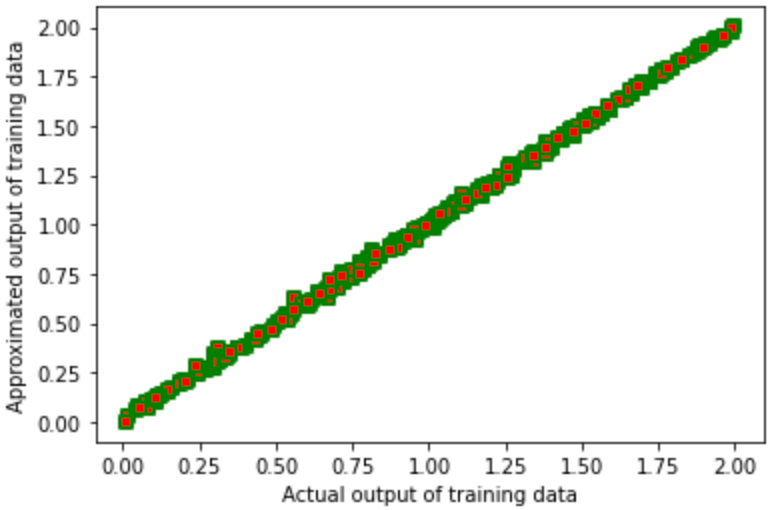
\includegraphics[width=0.8\linewidth]{Scatt.png}
    \captionsetup{justification=centering}
    \caption{Scatter plot of actual output vs model obtained output of training data}
\end{figure}

\subsection{Observations}
\begin{itemize}
    \item As the number of epochs increases, the average error decreases. After a point, the output just oscillates around the local optimum.
    \item Train average loss: 0.00167
    \item Test average loss: 0.00114
    \item The scatter plot showa that the data points almost lie along the $x=y$ line, showing the model has learnt well.
    \item The final plot obtained at 2000 epochs almost resembles the actual function plot, except it is more sharper at the edges.
    \item The validation loss varies with the epochs as follows:
    \subitem Validation average loss at epoch 0000: 0.217057
    \subitem Validation average loss at epoch 0100: 0.106351
	\subitem Validation average loss at epoch 0200: 0.050664
	\subitem Validation average loss at epoch 0300: 0.005119
	\subitem Validation average loss at epoch 0400: 0.006670
	\subitem Validation average loss at epoch 0500: 0.002086
	\subitem Validation average loss at epoch 0600: 0.001214
	\subitem Validation average loss at epoch 0700: 0.001714
	\subitem Validation average loss at epoch 0800: 0.001274
	\subitem Validation average loss at epoch 0900: 0.001025
	\subitem Validation average loss at epoch 1000: 0.000955
	\subitem Validation average loss at epoch 1100: 0.000678
	\subitem Validation average loss at epoch 1200: 0.000656
	\subitem Validation average loss at epoch 1300: 0.000648
	\subitem Validation average loss at epoch 1400: 0.000698
	\subitem Validation average loss at epoch 1500: 0.000476
	\subitem Validation average loss at epoch 1600: 0.003656
	\subitem Validation average loss at epoch 1700: 0.000401
	\subitem Validation average loss at epoch 1800: 0.000398
	\subitem Validation average loss at epoch 1900: 0.000314
	\item Final Train average loss: 0.00041
	\item Final Test average loss: 0.00031
\end{itemize}


\section{Classifying Image Data}

The images in the dataset given to us have been mapped to features of dimension 60. 
The features are then fed into our Multi Layer Feed Forward Neural Network model to classify the images into five 
distinct classes. 

\subsection{Hyper Parameter Optimization}

We tune the 

\subsection{Implementation Details:}

To prevent the model from overfitting (blah blah blah)


\subsection{Results}


\subsection{Observations}
raining data, to see how well the training data learns with multiple epochs. We observe that the loss steeply drops within the first few epochs and them asymptotically reaches to a value after which it is not able to learn much, and oscillates around the found local optimum.

\end{document}
